%!TEX root = ../thesis.tex

From the 1970s to the early 1990s, \gls{CMC} was largely limited to specialised communities, with technologies such as ARPANET designed with military and research purposes foremost in mind \cite{thorne_computer-mediated_2008}. As the Internet user\hyp{}base gradually diversified to include university staff and students, as well as select members of the private sector, \gls{CMC} became progressively more social in nature. By the early 1980s, linguists were researching both synchronous (i.e. chat) and asynchronous (e.g. bulletin boards, email) digital environments \cite[e.g.][]{carey_paralanguage_1980,myers_anonymity_1987,pullinger_chit-chat_1986}.

%todo: copy edit
This early body of research posited enduring representations of computer\hyp{}mediated and online environments \cite{postmes_formation_2000}. Often articulated was the \emph{reduced-cues perspective} \cite{thorne_computer-mediated_2008}, which argued that \gls{CMC} was a `lean' or `low\hyp{}bandwidth mode', stripped of the kinds of context available in face\hyp{}to\hyp{}face settings. Due to the observation that `social cues are filtered out in on\hyp{}line settings' \cite[p.~81]{parks_making_1996}, for instance, it was argued that complex corporate information was better suited to face\hyp{}to\hyp{}face transmission, due to the comparative `richness' of the face\hyp{}to\hyp{}face \gls{mode}. The main utility of \gls{CMC} was as a way of transmitting large sets of quantitative data \cite{daft_information_1983}. Similarly, in social scenarios, Parks and Floyd contended that the unavailability of `information regarding physical appearance' (1996, p.~84) stymied the potential for \glslink{member}{users} to build meaningful social relationships online.

%todo: fix collins 1992

Given the novel mixture of intimacy and detachment occurring during text\hyp{}based \gls{CMC} \cite{king_researching_1996}, research into the affordance of anonymity and its ramifications also proved major themes of early literature \cite{tanis_two_2007}. It was commonly argued until as late as the mid 1990s that anonymous \gls{CMC} was inherently genderless and egalitarian, due to the difficulty of verifying the identity and credentials of participants \cite{herring_computer-mediated_2001}. Related was the idea that people online were able to locate communicative partners based on shared interests and values, unbound by geographical location, with the potential consequence of more meaningful exchanges. On the other hand, many theorists argued that participants' anonymity allowed for reduced inhibitions, causing an increase in hostile discourses, or \emph{flaming} (Collins, 1992). \textcite{kiesler_social_1984} contended that flaming arose due to a lack of audience feedback, an inability to control or sanction those who transgress community rules, and `depersonalization' stemming from an absence of non\hyp{}verbal communication. \textcite[p.~7]{kim_verbal_1991} concurred, stating that in \gls{CMC}, participants were more likely `to abuse, make offensive comments, or criticize sharply'.

%todo: robyn doesn't like the brackets explaining adapted, reproduced etc.
%todo: signpost shift from describing typological perspectives to evaluation of them
During this period, some scholars aimed to classify different types of \gls{CMC} modes, or the kinds of behaviours exhibited by interactants therein. \textcite{crowston_reproduced_2000} argued that modes of \gls{CMC} can be understood from the perspective of genre theory. They found that for the most part, online genres of interaction may be \emph{reproduced} from pre-existing online antecedents (for example, online books and academic articles) or \emph{adapted} from offline antecedents into new genres (where, for example, hyperlinking creates new ways of browsing collections of texts). \emph{Novel} genres with no identifiable antecedent, such as website homepages and search engine listings, were also described. Interactive websites such as \glslink{forum}{online discussion forums} are also conceptualised as \emph{novel}, bearing little resemblance to pre-existing offline genres. \textcite{burnett_information_2000} provided an early typology of types of behaviour within novel interactive genres, noting the potential for non\hyp{}interactive lurking, and dividing active participation into hostile (flaming, trolling, etc.) and collaborative (humour, announcements, gossip, etc.) types (see Figure \ref{fig:burnett}). Though perspectives on early \gls{CMC} were variously optimistic or pessimistic, common to most was a treatment of \gls{CMC} under a \emph{deficit model}, where online interactions were considered inherently impoverished when compared to face\hyp{}to\hyp{}face modes. Burnett's typology is a good example of the implicitness of the deficit model in early research---indeed, it is difficult to imagine a researcher proposing such a reductive classificatory scheme to account for all offline human behaviour.

\begin{figure}[htb]
\centering
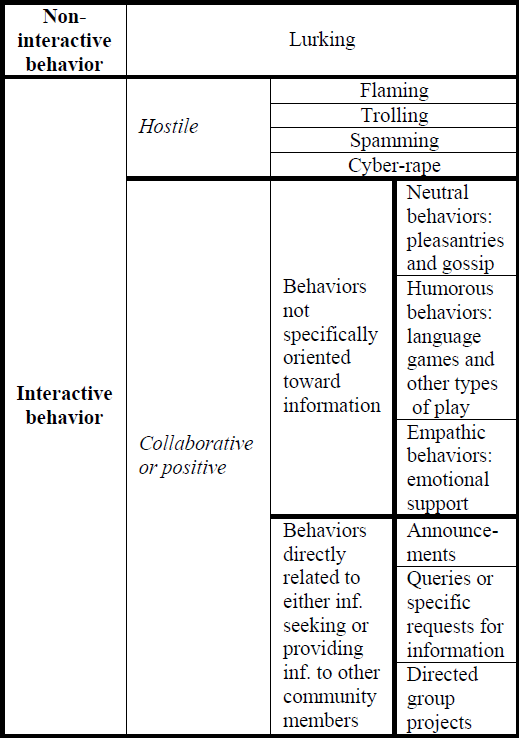
\includegraphics[width=0.45\textwidth]{../images/burnett.png}
\caption[Burnett's typology of online behaviour]{Burnett's typology of online behaviour (2000)}
\label{fig:burnett}
\end{figure}

\subsection{The changing face of \glsfmtshort{CMC}}

Between the mid 1990s and the mid 2000s, the nature of \gls{CMC}---and consequently, \gls{CMC} research---underwent a period of rapid change. As the result of a number of interwoven factors (the growing affordability of home computers; increasingly digital literacy; the development of early social network sites, etc.) the landscape of the Internet shifted from being primarily static and text\hyp{}based to dynamic, multimodal and participatory in nature \cite{herring_discourse_2011,lindholm_identity_2012}. The three currently most popular websites according to \emph{Alexa} in 2016 (\emph{Google}, \emph{YouTube} and \emph{Facebook}) exemplify this shift, in that each allows a great deal of user\hyp{}input and provides content in textual, audio and graphic modes. \textcite{herring_discourse_2011} reimagines the typology of familiar, adapted and new genres proposed by \textcite{crowston_reproduced_2000} to relate the dominant text types of `Web 2.0' to those that came before. Importantly, she notes that web genres can shift toward new\slash emergent as they mature, gaining features and responding to users' needs.

\subsubsection{Revisions of key claims in CMC research}

The profound nature of the shift to `Web 2.0' has meant that much early \gls{CMC} literature has now lost some of its relevance or explanatory power. Research into email messages is problematised by the fact that social media has overtaken email as the \gls{CMC} mode of choice for most digitally literate citizens \cite{thorne_computer-mediated_2008}, and by increasingly blurred boundaries between synchronous and asynchronous \glspl{mode}, such as email and instant messenger services. Similarly, the anonymity posited as critical to the discourse of early \gls{CMC}, while still possible, is no longer the norm: on social networking sites such as Facebook, \glslink{member}{users} communicate through personal accounts, disclosing their identities as they communicate and often even rendering the communication viewable to family and friends \cite{boyd_social_2007}. Furthermore, given that social networking sites are multimodal, and often contain a mixture of synchronous and asynchronous interactions, research informed by a characterisation of the Internet as fundamentally text\hyp{}based, or dealing exclusively with synchronous or asynchronous communication, is of limited usefulness for researchers of contemporary, often multimodal, \gls{CMC}.\endnote{For example, the myriad studies of communication on \emph{Usenet}---the text\hyp{}only Internet communication system in which many of the social elements of \gls{CMC} were first popularised---have been made largely redundant by the decommissioning of Usenet servers in 2010 \cite[e.g.][]{berge_computer-mediated_1995,eklundh_use_1994,jaffe_gender_1995}. That said, researchers have noted that despite greater bandwidth and the potential for multimodal interaction, in many respects, \gls{CMC} has remained surprisingly text\hyp{}based.}

In addition to the problem of reduced applicability, the findings of earlier research have since been challenged by research from the previous two decades \cite{herring_computer-mediated_2001,postmes_formation_2000}. As early as the mid 1990s, the characterisation of \gls{CMC} as impersonal, ineffective and hostile had come into question: \textcite{walther_computer-mediated_1996} argued that many early findings were caused by researchers' placing time restrictions on the observed \gls{CMC} interactions. If \gls{CMC} interactions are given unlimited time, Walther contends, they can achieve the same level of depth as face\hyp{}to\hyp{}face scenarios, both in terms of task\hyp{}completion and in the development of social relationships. In fact, Walther notes the potential for \emph{hyperpersonal} interaction in CMC: due to an optimised presentation of the self \cite[now often called \emph{self\hyp{}curation}; see][]{van_kleek_self_2015}, as well as idealisation of the Other, \gls{CMC} groups were found to be more polite and intimate than a face\hyp{}to\hyp{}face counterpart. Walther thus recognises two critical facts about interaction online: first, computer\hyp{}mediated interaction can be more candid than what could be observed in a comparable face\hyp{}to\hyp{}face setting; second, relationships develop in \gls{CMC} just as they do offline, necessitating longitudinal research. 

%From this perspective, aside from the slower pace of interactions, synchronous text\hyp{}based \gls{CMC} and face\hyp{}to\hyp{}face communication can be conceptualised as fundamentally similar in nature \cite{osullivan_reconceptualizing_2003,walther_interpersonal_1994,wu_is_2013}. The rapid increase in access to \gls{CMC} since this study 

The notion of a genderless and egalitarian Internet has faced similar scrutiny: \gls{CMC} research has shown that gender in anonymous, text\hyp{}only \gls{CMC} is often encoded by the \glslink{lexicogrammar}{lexicogrammatical} choices of the writer, as well as through the use of gendered discourse strategies such as assertiveness, politeness and aggression \cite{herring_gender_2000}. Likewise, education level is conveyed through vocabulary and complexity of message structure, and age through the discussion of interests and life experiences \cite{herring_computer-mediated_2001}. These findings echo the \glslink{SFL}{systemic-functional} notion that \emph{context is in text}, rather than around it, and can thus be reconstructed from linguistic analysis \cite[see Section \ref{sect:sfl}, as well as][]{eggins_introduction_2004}. Finally, research from the perspective of \gls{CDA} has questioned the notion of an egalitarian Internet at two separate levels. At the level of discourse, newer studies show that complex and rigid power structures exist online, even in low\hyp{}bandwidth \glspl{forum} and discussion lists \cite[e.g.][]{stommel_online_2010}. More broadly, contemporary theorists acknowledge that the landscape of \gls{CMC} has `inherit[ed] power asymmetries from the larger historical and economic context of the Internet', with a notable over-representation of English speaking, white males positioned as moderators, webmasters, and page creators \cite[p.~12]{herring_computer-mediated_2001}.

%Data and metadata are commodities: a main source of revenue for micro-blogging website Twitter is its \emph{Firehose}---an API that allows customers access to 500 million tweets per day. Researchers have attempted to mine tweets to detect natural disasters; to play the stockmarket; to aggregate content for entertainment websites. Each of these tasks requires the extraction of information from natural language.

\subsection{Contemporary CMC and its affordances for research}

%Though the Web is becoming more and more multimodal, methods for analysing human behaviour based on creation and consumption of multimodal content are only emerging. Multimodal content is very difficult to process automatically---typically, a great deal of manual effort is needed to transform multimodal content into data, and from data into insight. Plain text and metadata, however, are easier to transform into data, easier to annotate, and easier to search.

%todo: possible conflict between gruba and robyn re: future proofing ... i've deleted 'By 2016'
\gls{CMC} has now become become a central component of daily life, accounting for an ever\hyp{}increasing proportion of all human communication. Today, \gls{CMC} is used to contact those already close to us, rather than like\hyp{}minded strangers. Instead of well\hyp{}defined sessions of \gls{CMC} at a home computer, \gls{CMC} is now dispersed through work, travel and social occasions, and facilitated by an interconnected ecosystem of smartphones, tablets, laptops and desktop computers. Media convergence has led to new genres of communication, between journalists and readers, or companies and customers. The current Web therefore provides language examples that cannot be obtained through other means \cite{harvey_disclosures_2012}, or which have no antecedent in face\hyp{}to\hyp{}face discourse \cite{herring_discourse_2011}. As such, analysis of \gls{CMC} texts becomes necessary for investigation of many longstanding aims of linguistic research, including how language changes or evolves, how language is used to form and attend to social relationships \cite{canary_relationship_2015}, and\slash or how language is used to construe the human experience of the world.

\section{Healthcare and online communities}

% bit of a jump here ... 
Health discourse, in some form or another, is a large part of the landscape of contemporary \gls{CMC}---72 per cent of adult Internet users in the U.S. report having searched for health\hyp{}related content online \cite{fox_health_2013,fox_social_2014}. As mentioned in Chapter \ref{chap:intro}, talk about health covers a spectrum of registers \cite[in the systemic-functional sense\textemdash{}see][as well as Section \ref{sect:sfl}]{halliday_introduction_2004}. Ideationally, healthcare is a key topic online, with information about every conceivable symptom, illness and treatment strategy readily available through search engine results. Textually, health is represented in every popular \gls{mode} of \gls{CMC}, including wikis, blogs, online news, chatrooms, static information pages and mobile apps. Interpersonally, online health information targeting \glspl{consumer}%
\endnote{Interpersonally, not all health information online targets consumers---there are also sites with information for health professionals, academics, and so forth. These, however, are not relevant to the thesis.}
may be authored by governments, non\hyp{}profit organisations, health professionals, researchers, journalists, or, importantly, by healthcare consumers themselves. The latter of these---personal experiences with healthcare, authored by those living with health problems, and those who care for them, have significant public demand: a quarter of surveyed U.S. adults report specifically seeking out \glspl{consumer}' subjective accounts of their experiences with illnesses and journeys through healthcare systems \cite{fox_social_2014}.

Much consumer\hyp{}generated talk about health goes on inside dedicated online communities\textemdash{}that is, `mediated social spaces in the digital environment that allow groups to form and be sustained primarily through ongoing virtual communication processes' \cite[p.~986]{shen_effects_2013}. These communities most commonly exist within social networking sites (e.g. Facebook groups, Subreddits) or within bulletin board\slash \gls{forum} platforms\textemdash{}text-based \glspl{mode} of \gls{CMC} where registered \glslink{member}{users} can create and reply to \glspl{thread}. In academic literature and beyond, health\hyp{}oriented \glspl{forum} have been conceptualised as \glsxtrfullpl{OSG}\textemdash{}an online permutation of more traditional support networks for people living with health problems, or for those who care for them.

\glslink{forum}{Forum}\hyp{}based online communities and \glspl{OSG} have long been used as data sources for linguistic research due to their size, ubiquity and the ease with which they can be accessed: access to \glspl{forum} is round\hyp{}the\hyp{}clock and global; recording and transcription are unnecessary; and in many cases linguistic data is accompanied by rich, well\hyp{}structured demographic metadata \cite{leech_new_2006}. In general, empirical studies have shown that when contrasted with face\hyp{}to\hyp{}face equivalents, online communities have fewer barriers to entry, higher dropout rates and a comparatively high proportion of peripheral membership---that is, a greater rate of inexperienced or new members, compared to longstanding veterans \cite{sandaunet_challenge_2008,zhang_peripheral_2001}. That said, the efficacy of comparisons and contrasts between face\hyp{}to\hyp{}face and computer\hyp{}mediated communities has recently been questioned, as daily life becomes increasingly mediated by and merged with digital technologies \cite{wu_is_2013}. Indeed, a great number of users of \glspl{OSG} have never attended the offline antecedent of the \gls{mode}.

Linguists have paid attention to the central role played by language in online communities and \glspl{OSG}. It has long been argued by researchers that the limited semiotic resources available in many online environments (chiefly, a lack of physical co\hyp{}presence) makes language the most suitable resource for identity construction and role\hyp{}relationship negotiation \cite{thorne_computer-mediated_2008}. As \textcite[p.~303]{lam_language_2008} notes, `language practices are instrumental in creating the norms of behavior of particular online groups and how these norms function to provide sociability, support, information, and a sense of collective identity'. A similar perspective is provided by \textcite{postmes_formation_2000}, who argues that social identity issues have a stronger presence in \gls{CMC} environments, due to the de\hyp{}individuation that occurs in part due to reduced cues online. Because \glspl{OSG} facilitate intra\hyp{}consumer exchange, and because of the centrality of language to this task, the main thrust of linguistic online community and \gls{OSG} research has been toward language as an interpersonal, rather than an ideational resource---that is, toward the ways in which language is used to enact social relationships, rather than as a means of construing reality. Many studies have focussed on differences in communicative practices over the course of membership\textemdash{}most typically, on how newcomers position themselves as legitimate prospective members whose contributions deserve replies, and how longer\hyp{}term members represent their expertise and construct\slash reinforce normative community values. In the sections that follow, I review key \glspl{theme} in linguistic accounts of interpersonal meaning\hyp{}making in online communities, with preference given to \gls{forum}\hyp{}based or health\hyp{}oriented communities where available.

%In health contexts, the centrality language provides an attractive possibility for research into \gls{consumercentred} care, which similarity shares an interest in interpersonal, rather than ideational meaning\hyp{}making.